\chapter{LPM\_ROM \& LPM\_RAM 实验}
\section{实验内容}

本实验分为两个子实验:

\begin{itemize}
    \item LPM\_ROM 实验
    \item LPM\_RAM 实验
\end{itemize}

要求会初始化/读/写存储器。

\section{实验原理}

\subsection{LPM\_ROM}

\begin{figure}[H]
\centering
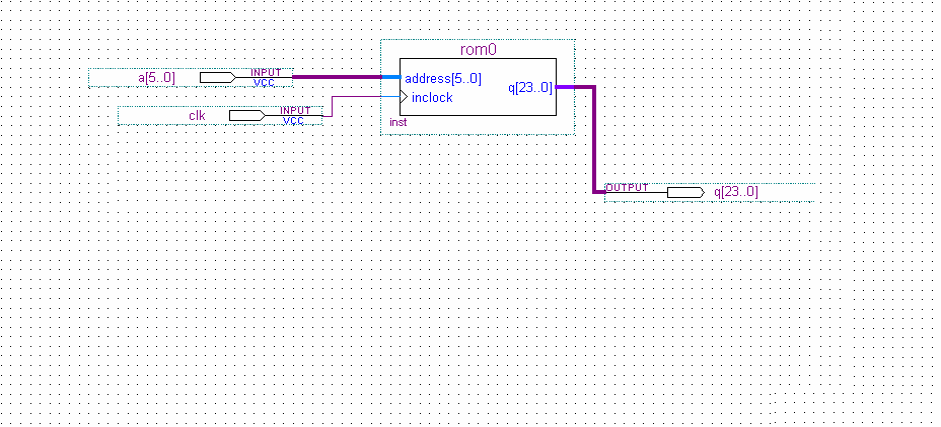
\includegraphics[width=\textwidth]{images/prin2_1.png}
\caption{LPM\_ROM}
\label{fig:prin2_1}
\end{figure}

如图\ref{fig:prin2_1},由LPM\_ROM 组成,地址线 6 位,数据线 24 位。

\subsubsection{输入信号}

\begin{itemize}
    \item clk
    
    时钟信号,稳定的等间隔方波信号。

    可由外部控制的输入信号。
    
    \item a[5..0]
    
    地址信号,6 位,用于存储器寻址。
    
    可由外部控制的输入信号。
    
\end{itemize} 

\subsubsection{输出信号}

\begin{itemize}
    \item q[23..0]
    
    数据信号,24 位,存储器输出的数据信号。
    
\end{itemize}

\subsection{LPM\_RAM}

\begin{figure}[H]
\centering
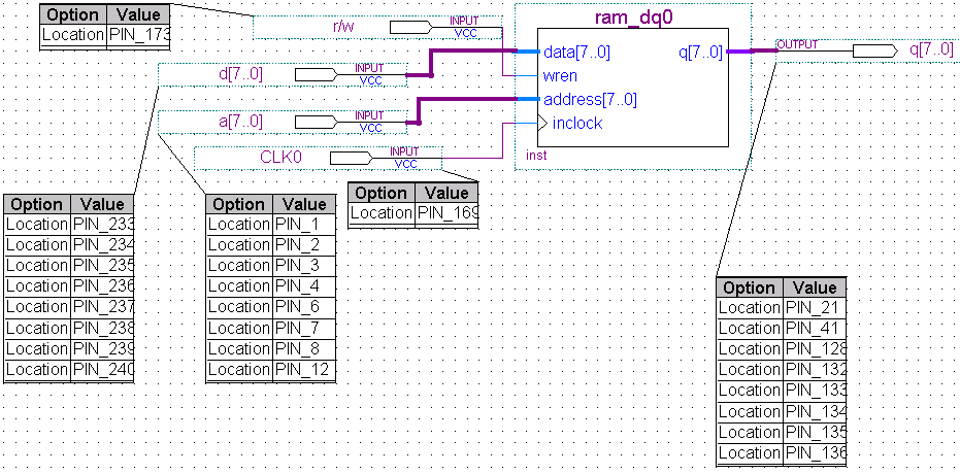
\includegraphics[width=\textwidth]{images/prin2_2.png}
\caption{LPM\_RAM}
\label{fig:prin2_2}
\end{figure}

如图\ref{fig:prin2_2},由LPM\_RAM 组成,地址线 8 位,数据线 8 位。

\subsubsection{输入信号}

\begin{itemize}
    \item CLK0
    
    时钟信号,稳定的等间隔方波信号。

    可由外部控制的输入信号。
    
    \item r/w
    
    读写控制信号,控制存储器当前是读模式还是写模式。
    
    \item a[7..0]
    
    地址信号,8位,用于存储器寻址。
    
    可由外部控制的输入信号。

    \item d[7..0]
    
    数据信号,8位,用于写存储器时输入数据。
    
    可由外部控制的输入信号。
    
\end{itemize} 

\subsubsection{输出信号}

\begin{itemize}
    \item q[7..0]
    
    数据信号,8 位,存储器输出的数据信号。
    
\end{itemize}

\section{实验任务与实验步骤}

\subsection{LPM\_ROM}

\begin{enumerate}
    \item 按照原理图 \ref{fig:prin2_1} 连接电路图,然后编译。
    
    \begin{enumerate}
        \item 配置 LPM\_ROM
        
        \begin{itemize}
            \item 输出数据字长:24 位。
            \item 存储器可寻址单元数:64 字。
            \item 禁用输出端口。
            \item 创建对应大小的 ROM\_5.mif 文件初始化 ROM。
            
            \begin{figure}[H]
            \centering
            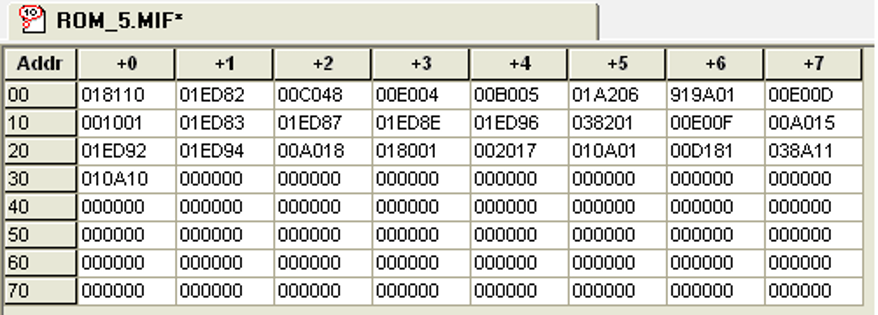
\includegraphics[width=\textwidth]{images/init2_1.png}
            \caption{LPM\_ROM 初始化数据}
            \label{fig:init2_1}
            \end{figure}
            
            \item 启用内建的储存器内容编辑器 \footnote{Allow In-System Memory Content Editor to capture and update content independently of the system clock: 允许系统内建的储存器内容编辑器异步地跟踪与更新储存器内容},实例名为 rom3。
        \end{itemize}
        
    \end{enumerate}
    
    \item 将输入输出器件绑定到对应的引脚上,然后重新编译。
    
    \begin{table}[H]
        \centering
        \begin{tabular}{|c|c|c|}
            \hline
            名称 & 引脚号 & 备注 \\
            \hline
            clk & 240 & Key 8 \\
            \hline
            a[0] & 1 & Key 1 \\
            \hline
            a[1] & 2 & Key 1 \\
            \hline
            a[2] & 3 & Key 1 \\
            \hline
            a[3] & 4 & Key 1 \\
            \hline
            a[4] & 6 & Key 2 \\
            \hline
            a[5] & 7 & Key 2 \\
            \hline
            q[0] & 21 & 数码 3 \\
            \hline
            q[1] & 41 & 数码 3 \\
            \hline
            q[2] & 128 & 数码 3 \\
            \hline
            q[3] & 132 & 数码 3 \\
            \hline
            q[4] & 133 & 数码 4 \\
            \hline
            q[5] & 134 & 数码 4 \\
            \hline
            q[6] & 135 & 数码 4 \\
            \hline
            q[7] & 136 & 数码 4 \\
            \hline
            q[8] & 137 & 数码 5 \\
            \hline
            q[9] & 138 & 数码 5 \\
            \hline
            q[10] & 139 & 数码 5 \\
            \hline
            q[11] & 140 & 数码 5 \\
            \hline
            q[12] & 141 & 数码 6 \\
            \hline
            q[13] & 158 & 数码 6 \\
            \hline
            q[14] & 159 & 数码 6 \\
            \hline
            q[15] & 160 & 数码 6 \\
            \hline
            q[16] & 161 & 数码 7 \\
            \hline
            q[17] & 162 & 数码 7 \\
            \hline
            q[18] & 163 & 数码 7 \\
            \hline
            q[19] & 164 & 数码 7 \\
            \hline
            q[20] & 165 & 数码 8 \\
            \hline
            q[21] & 166 & 数码 8 \\
            \hline
            q[22] & 167 & 数码 8 \\
            \hline
            q[23] & 168 & 数码 8 \\
            \hline
        \end{tabular}
        \caption{LPM\_ROM 实验引脚表}
        \label{tab:pin2_1}
    \end{table}
    
    
    \item 下载到实验设备上。
    \item 调整为工作模式 0。
    \item 观察实验现象。
    
    \begin{itemize}
        \item Key 1, 2 (D1 - D8)
        
        控制地址,低 6 位 (D1 - D6) 有效。
        
        \item Key 8
        
        控制时钟。
        
        \item 数码管 3 - 8
        
        输出的数据,24 位全有效。
        
    \end{itemize}
    \item 绘制仿真波形图。
\end{enumerate}

\subsection{LPM\_RAM}

\begin{enumerate}
    \item 按照原理图 \ref{fig:prin2_2} 连接电路图,然后编译。
    
    \begin{enumerate}
        \item 配置 LPM\_RAM
        
        \begin{itemize}
            \item 输出数据字长:8 位。
            \item 存储器可寻址单元数:256 字。
            \item 禁用输出端口。
            \item 创建对应大小的 5\_RAM.mif 文件初始化 RAM。
            
            \begin{figure}[H]
            \centering
            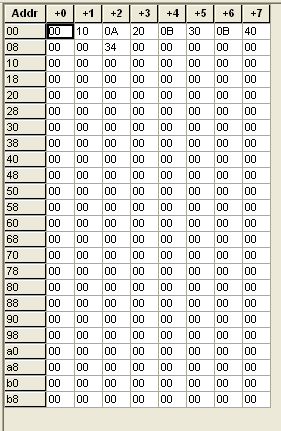
\includegraphics{images/init2_2.png}
            \caption{LPM\_RAM 初始化数据}
            \label{fig:init2_2}
            \end{figure}
            
            \item 启用内建的储存器内容编辑器,实例名为 ram1。
        \end{itemize}
        
    \end{enumerate}
    
    \item 将输入输出器件绑定到对应的引脚上,然后重新编译。
    
    \begin{table}[H]
        \centering
        \begin{tabular}{|c|c|c|}
            \hline
            名称 & 引脚号 & 备注 \\
            \hline
            CLK0 & 169 & Key 7 \\
            \hline
            r/w & 173 & Key 8 \\
            \hline
            a[0] & 1 & Key 3 \\
            \hline
            a[1] & 2 & Key 3 \\
            \hline
            a[2] & 3 & Key 3 \\
            \hline
            a[3] & 4 & Key 3 \\
            \hline
            a[4] & 6 & Key 4 \\
            \hline
            a[5] & 7 & Key 4 \\
            \hline
            a[6] & 8 & Key 4 \\
            \hline
            a[7] & 12 & Key 4 \\
            \hline
            d[0] & 233 & Key 2 \\
            \hline
            d[1] & 234 & Key 2 \\
            \hline
            d[2] & 235 & Key 2 \\
            \hline
            d[3] & 236 & Key 2 \\
            \hline
            d[4] & 237 & Key 2 \\
            \hline
            d[5] & 238 & Key 2 \\
            \hline
            d[6] & 239 & Key 2 \\
            \hline
            d[7] & 240 & Key 2 \\
            \hline
            q[0] & 21 & 数码 7 \\
            \hline
            q[1] & 41 & 数码 7 \\
            \hline
            q[2] & 128 & 数码 7 \\
            \hline
            q[3] & 132 & 数码 7 \\
            \hline
            q[4] & 133 & 数码 8 \\
            \hline
            q[5] & 134 & 数码 8 \\
            \hline
            q[6] & 135 & 数码 8 \\
            \hline
            q[7] & 136 & 数码 8 \\
            \hline
        \end{tabular}
        \caption{LPM\_ROM 实验引脚表}
        \label{tab:pin2_2}
    \end{table}
    
    
    \item 下载到实验设备上。
    \item 调整为工作模式 1。
    \item 观察实验现象。
    
    \begin{itemize}
        \item Key 1, 2 (数码 1, 2)
        
        控制输入数据,8 位全有效。
        
        \item Key 3, 4 (数码 3, 4)
        
        控制地址,8 位全有效。
        
        \item Key 7 (D15)
        
        控制时钟。
        
        \item Key 8 (D16)
        
        控制 r/w 读写开关。
        
        \item 数码管 7, 8
        
        输出的数据,8 位全有效。
        
    \end{itemize}
    \item 绘制仿真波形图。
\end{enumerate}


\section{实验结果分析}

\subsection{实验电路图}

根据原理图 \ref{fig:prin2_1} 绘制实验电路图 \ref{fig:bdf2_1}。

\begin{figure}[H]
\centering
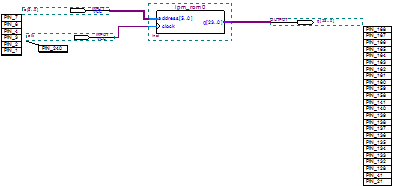
\includegraphics[width=\textwidth]{images/bdf2_1.png}
\caption{LPM\_ROM 实验电路图}
\label{fig:bdf2_1}
\end{figure}

根据原理图 \ref{fig:prin2_2} 绘制实验电路图 \ref{fig:bdf2_2}。

\begin{figure}[H]
\centering
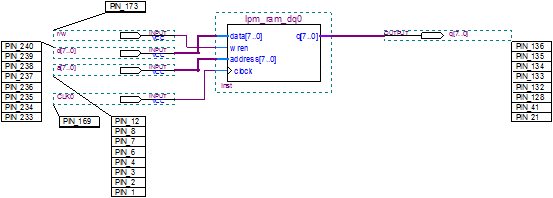
\includegraphics[width=\textwidth]{images/bdf2_2.png}
\caption{LPM\_RAM 实验电路图}
\label{fig:bdf2_2}
\end{figure}

\subsection{仿真波形图}

利用 Quartus II 产生仿真波形图 \ref{fig:wave2_1}。

\begin{figure}[H]
\centering
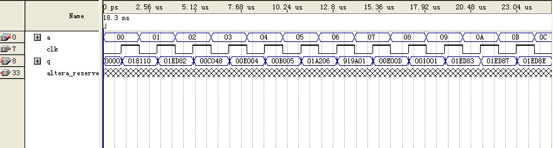
\includegraphics[width=\textwidth]{images/wave2_1.png}
\caption{LPM\_ROM 实验 仿真波形图}
\label{fig:wave2_1}
\end{figure}

利用 Quartus II 产生仿真波形图 \ref{fig:wave2_2}。

\begin{figure}[H]
\centering
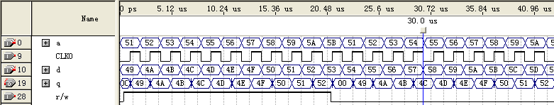
\includegraphics[width=\textwidth]{images/wave2_2.png}
\caption{LPM\_RAM 实验 仿真波形图}
\label{fig:wave2_2}
\end{figure}

\subsection{思考题}

\begin{enumerate}
    \item 如何建立 lpm\_ram\_dq 的数据初始化?
    
    \textbf{答}:需要创建一个初始化文件并在储存器中配置该初始化文件。
    
    \begin{enumerate}
        \item 创建 Hexadecimal File (Intel-Format) (.MIF) 文件。
        \item 设定大小,然后进行初始化赋值。
        \item 在储存器的属性中配置该初始化文件。
    \end{enumerate}
    
\end{enumerate}
